\section{Model-based evaluation of the policy}

\begin{frame} 
\mode<presentation>{
    \begin{center} \huge
        \secname
    \end{center}  
    }
    \begin{center} 
    Model-based $\corresponds$ offline-planning.\\
    We are told everything about the environment, so we can simulate ``looking ahead'' and determine if one policy is better than another.
    \end{center}
\end{frame}

\subsection{The Bellman equation}

\begin{frame}\frametitle{\subsecname}

The Bellman equation relates the value of a state with the values of its successor states, given some policy $\pi$.

The policy is fixed beforehand, i.e. $V$ ``follows'' the policy $\pi$.

\end{frame}

\begin{frame}\frametitle{\subsecname}


\slidesonly{\vspace{-4mm}}

	\begin{align}
	V^\pi_i 
    \only<1>{
    =\;&
	\E \Big\lbrack
	\sum_{t=0}^{\infty} \gamma^t \; \overbrace{r(\vec x^{(t)}, \vec a^{(t)})}^{\substack{\text{shorthand}\\=: r^{(t)}}} \;\Big|\; \vec x^{(0)} := \vec x_i
	\Big\rbrack\,, \; i=1,\ldots,S\\
	=\;& 
	\E \Big\lbrack
	\sum_{t=0}^{\infty} \gamma^t r^{(t)} \;\Big|\; \vec x^{(0)} := \vec x_i
	\Big\rbrack\\
	=\;& 
	\E \Big\lbrack
	\gamma^0 \kern-1.5ex \underbrace{r^{(0)}}_{\substack{\text{immediate}\\ \text{reward}}} \kern-1.5ex + \gamma^1 r^{(1)} + \gamma^2 r^{(2)}+\ldots\;\Big|\; \vec x^{(0)} := \vec x_i
	\Big\rbrack\\
	=\;& 
	\E \Big\lbrack
	r^{(0)} + 
	\underbrace{\gamma \big( r^{(1)} + \gamma r^{(2)}+\ldots\big)
	}_{\substack{
	\text{discounted value of}\\ \text{successor state}}}\;\Big|\; \vec x^{(0)} := \vec x_i
	\Big\rbrack\\}
    \only<1,2>{
	=\;&
	\E \Big\lbrack
	r^{(0)} + 
	\gamma V^\pi(\vec x^{(1)})\;\Big|\; \vec x^{(0)} := \vec x_i
	\Big\rbrack
    }
    \only<2>{
	\intertext{split ``expectation of sum'' into ``sum of expectations'':}
	=\;& 
	\E \Big\lbrack
	r^{(0)} \;\Big|\; \vec x^{(0)} := \vec x_i
	\Big\rbrack
	+
	\E \Big\lbrack
	{\color{red}\gamma} V^\pi( \vec x^{(1)})\;\Big|\; \vec x^{(0)} := \vec x_i
	\Big\rbrack\\
	=\;& 
	\E \Big\lbrack
	r^{(0)} \;\Big|\; \vec x^{(0)} := \vec x_i
	\Big\rbrack
	+
	{\color{red}\gamma}\,
	\E \Big\lbrack
	 V^\pi( \vec x^{(1)})\;\Big|\; \vec x^{(0)} := \vec x_i
	\Big\rbrack
    }
	\end{align}
	
\end{frame}

\begin{frame}\frametitle{\subsecname~(cont'd)}

\slidesonly{\vspace{-5mm}}

\mode<presentation>{
	\begin{align}
		V^\pi_i =\;& 
		\E \bigg\lbrack
		r^{(0)} \;\Big|\; \vec x^{(0)} := \vec x_i
		\bigg\rbrack
		+
		\gamma\,
		\E \bigg\lbrack
		 V^\pi( \vec x^{(1)})\;\Big|\; \vec x^{(0)} := \vec x_i
		\bigg\rbrack
	\end{align}

\only<1-3>{
Recall:
\begin{itemize}
\item[] states $\vec x \in \{ \vec x_1, \ldots, \vec x_S\}$, 
actions $\vec a \in \{ \vec a_1, \ldots, \vec a_A\}$,\\
reward function $r(\vec x_i, \vec a_k)$,
\item[]
transition model ${\color{trans} P(\vec x_j | \vec x_i, \vec a_k)}$ and
policy ${\color{policy} \pi(\vec a_k | \vec x_i)}$
\end{itemize}
}
}

\question{What does the $\E \lbrack \cdot \rbrack$ boil down to?}

\pause

\slidesonly{\vspace{-10mm}}

	\begin{align}
		V^\pi_i 
		&=& \visible<2->{
		\underbrace{
		{\color{policy} \sum_{k=1}^A \pi(\vec a_k \,|\, \vec x_i)}
			 {\color{reward} r(\vec x_i, \vec a_k)}
			 }_{\substack{\text{``controlled'' reward function }\\
			 \text{(immediate reward)} =: {\color{reward} r_i^\pi}}
			 }
		+
		}
		\visible<3->{
			 \underbrace{
			\gamma {\color{policy} \sum_{k=1}^A \pi(\vec a_k \,|\, \vec x_i)} {\color{trans}\smallsum{j=1}{S} 
				P(\vec x_j \,|\, \vec x_i, \vec a_k)} \kern-1.2ex
				\overbrace{V^\pi_j}^{=V^\pi(\vec x_j)}
				}_{\text{expected discounted value of successor state}} \\	
		&=& 
		}
		\visible<4->{
			\underbrace{{\color{policy} \smallsum{k=1}A 
				\pi(\vec a_k \,|\, \vec x_i)} 
				{\color{reward} r(\vec x_i, \vec a_k)}
			}_{\kern-4ex\text{``controlled'' reward function }
					{\color{reward} r_i^\pi}\kern-4ex}
			\;+\; \gamma {\color{trans} \smallsum{j=1}{S}}
			\underbrace{
				{\color{policy} \smallsum{k=1}A 
				\pi(\vec a_k \,|\, \vec x_i)} 
				{\color{trans} P(\vec x_j \,|\, \vec x_i, \vec a_k)}
			}_{\text{``controlled'' transition model }
					{\color{trans} P^\pi_{ij}}}  V^\pi_j
		}
	\end{align}
	
	\notesonly{
	Thus, the Bellman equation can be expressed using:
	
	\begin{equation}
	V^\pi_i
	= {\color{reward}\vec r^\pi_i} 
			+ \gamma {\color{trans}\vec P^\pi_{ij}} \vec v^\pi_{j}
	\end{equation}
	}
	\visible<4>{
	
	\mode<presentation>{
		$$
		\vec v^\pi
		= {\color{reward}\vec r^\pi} 
				+ \gamma {\color{trans}\vec P^\pi} \vec v^\pi
		$$
		}
	}
	
	
\end{frame}

\begin{frame}
	
	\begin{equation}
		\vec v^\pi
		= \; {\color{reward}\vec r^\pi} 
			+ \gamma {\color{trans}\vec P^\pi} \vec v^\pi \; =: \kern-3ex\overbrace{\hat B^\pi[\vec v^\pi]}^{\text{the Bellman operator}}\kern-3ex,
	\end{equation}
	
	where $\vec v^\pi \in \R^S$ is a vector containing all values $V^\pi(\vec x_{i})\;\forall i$,
	
	\begin{align}
		\quad \text{with}  \underbrace{ \left\{ \begin{array}{rcl} 
				{\color{reward}r^\pi_i} &\kern-1ex:=\kern-1ex& 
					{\color{policy} \smallsum{k=1}{A} 
					\pi(\vec a_k \,|\, \vec x_i)} \, 
					{\color{reward} r(\vec x_i, \vec a_k)} \\
				{\color{trans}P^\pi_{ij}} &\kern-1ex:=\kern-1ex& 
					{\color{policy}\smallsum{k=1}{A} 
					\pi(\vec a_k \,|\, \vec x_i)} \, 
					{\color{trans}P(\vec x_j | \vec x_i, \vec a_k)} \\
			\end{array} 
			\right.\kern-2ex}_{
				\text{``controlled'' models }
				{\color{reward}\vec r^\pi \in \R^S}
				\text{ and }{\color{trans}\vec P^\pi \in \R^{S \times S}}
			}
	\end{align}
	
\end{frame}

\subsection{Finding the value}

\begin{frame}\frametitle{Finding $\vec v^\pi$}

\mode<presentation>{
	$$
	\vec v^\pi
	= {\color{reward}\vec r^\pi} 
			+ \gamma {\color{trans}\vec P^\pi} \vec v^\pi
	$$
	
}
There are two approaches to finding $\vec v^\pi$:

\begin{enumerate}
\item[\ref{sec:findvanalytical} -] analytically
\item[\ref{sec:findviter} -] through fixed-point iteration
\end{enumerate}

\end{frame}

\subsubsection{Analytical solution of the Bellman equation}\label{sec:findvanalytical}

\begin{frame}\frametitle{Finding $\vec v^\pi$:~\subsubsecname}

Essentially solve for $\vec v^\pi$ (get \underline{all} $\vec v^\pi$ on one side):

	\begin{align}
		\vec v^\pi &= {\color{reward}\vec r^\pi} 
		+ \gamma {\color{trans}\vec P^\pi} \vec v^\pi \\
		\vec I~\vec v^\pi 
        &= {\color{reward}\vec r^\pi}
		+ \gamma {\color{trans}\vec P^\pi} \vec v^\pi
	\\
		\vec I~\vec v^\pi - \gamma {\color{trans}\vec P^\pi} \vec v^\pi
		&= {\color{reward}\vec r^\pi}
	\\
		\big(\vec I - \gamma {\color{trans}\vec P^\pi}\big) \vec v^\pi
		&= {\color{reward}\vec r^\pi}
	\\
	\vec v^\pi &= \big(\vec I 
			- \gamma {\color{trans}\vec P^\pi}\big)^{-1}
		 {\color{reward}\vec r^\pi}
	\end{align}
	
	\question{When is the term $\big(\vec I 
			- \gamma {\color{trans}\vec P^\pi}\big)$ invertible?}
		
\begin{enumerate}
\item $|\lambda_k| \leq 1$ for all eigenvalues 
				$\lambda_k$ of transition matrix ${\color{trans}\vec P^\pi}$
\item $\gamma < 1$
\item[$\Rightarrow$] it is always invertible
\end{enumerate}

\slidesonly{\vspace{-5mm}}

\question{Any disadvantages to the analytical solution?}\\

\pause 
- It could be very costly for very large state spaces.

\end{frame}


\subsubsection{Value iteration}\label{sec:findviter}

\begin{frame}\frametitle{Finding $\vec v^\pi$:~\subsubsecname}

Value iteration: a fixed-point iteration for finding $\vec v^\pi$

\begin{itemize}
\item A fixed point: $x=g(x)=g(g(\ldots g(x)\ldots))$\\

Example:
\begin{align}
    g(x) &= x^{2} - 3x + 4\\
    g(2) &= 2^{2} - 3\cdot 2 + 4 = 4 - 6 + 4 = 2
\end{align}

\item Fixed point iteration:
\begin{equation}
x^{(t+1)} = g(x^{(t)}), t=0,1,2,\ldots
\end{equation}
\end{itemize}

\begin{center}
    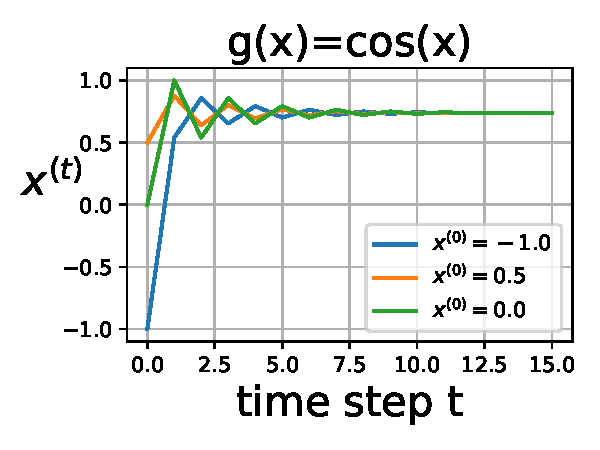
\includegraphics[height=3.5cm]{img/fixed_point_iter_cos} 
    \mode<article>{
    \captionof{figure}{
    Fixed point iteration example
    }
    \label{fig:fixedpointcos}
    } 
\end{center}

\end{frame}


\begin{frame}\frametitle{Finding $\vec v^\pi$:~\subsubsecname}
\mode<presentation>{
Value iteration: a fixed-point iteration for finding $\vec v^\pi$
}

\begin{equation}
	\vec {\tilde v}^{\pi (t+1)} = {\color{reward}\vec r^\pi} 
		+ \gamma {\color{trans}\vec P^\pi} \vec {\tilde v}^{\pi (t)} 
\end{equation}

\begin{itemize}
\item 
The ``~$\tilde{}$~'' is to denote that it has not necessarily converged 
at time step $t$
\item initialize $\vec {\tilde v}^{\pi (0)}$ with some state $\vec {\tilde v}^{\pi (0)} \in \R^{S}$
\item value iteration converges in the limit $t \rightarrow \infty$
\item The speed of convergence depends on $\gamma$
\end{itemize}

\question{How does convergence depend on $\gamma$?}

\pause 

\begin{itemize}
\item small $\gamma$: fast convergence
\item $\gamma \rightarrow 1$: slow convergence, slower than the analytical solution
\end{itemize}

\end{frame}


\begin{frame}\frametitle{Finding $\vec v^\pi$:~\subsubsecname}
    
\mode<presentation>{
\begin{equation}
	\vec {\tilde v}^{\pi (t+1)} = {\color{reward}\vec r^\pi} 
		+ \gamma {\color{trans}\vec P^\pi} \vec {\tilde v}^{\pi (t)} 
\end{equation}
}

\begin{itemize}
\item We start \emph{value iteration} assuming $\vec {\tilde v}^{\pi (0)}$ is the optimal value function
\item Use the one-step \emph{look-ahead} (i.e. next step) to work our way \emph{backwards}\\

	\begin{equation*}
		\hat B^\pi[\vec v^\pi] :=
		{\color{reward}\vec r^\pi} 
			+ \gamma {\color{trans}\vec P^\pi} \kern-1.7ex \underbrace{\vec v^\pi}_{\text{look-ahead}}
	\end{equation*}
\end{itemize}

\end{frame}

\begin{frame}\frametitle{Analytical solution vs. value iteration}

\mode<article>{
Analytical solution vs. value iteration:
}

\begin{itemize}
\item complexity: 
\begin{itemize}
\item Analytical solution: $O(S^{3})$
\item value iteration: $O(S^{2})$
\end{itemize}   
\item intermediate solutions of \emph{value iteration} don't necessarily belong to valid policies. We have to wait for convergence.
\end{itemize}

\end{frame}

\newpage

\subsubsection{Convergence of value iteration}


% -----------------------------------------------------------------------------
\begin{frame} \frametitle{\subsubsecname}
    
    \only<1,2>{
	\begin{block}{Contraction mapping}
		\small
		A mapping function $f(x)$ is a contraction with $0 < \gamma < 1$ if for any $x, x'$, $\lVert f(x) - f(x') \rVert \le \gamma \lVert x - x' \rVert$.
	\normalsize
	\end{block}
    
    \mode<article>{
    We specify this a little further:
    }
    }
    
    \only<2->{
	\begin{block}{Contraction mapping (in supremum norm)}
		\small
		A function $\hat B : \R^S \to \R^S$ is called a 
		{\em contraction mapping} 
		with Lipschitz constant\notesonly{\footnote{i.e. the function is continuous and the absolute value of the slope does not exceed some constant, which is a real number. That real number is the Lipschitz constant.}} $0 \leq \lambda < 1$ if 
		$\max\limits_{j} 
		\big|(\hat B[\tilde{\vec v}] - \hat B[\tilde{\vec w}])_j \big| 
		\;\leq\; \lambda \max\limits_{j} \big|\tilde v_j - \tilde w_j \big|,
		\forall \tilde{\vec v}, \tilde{\vec w} \in \R^S$.
	\normalsize
	\end{block}
	}
	\only<3>{ 
		\vspace{2mm}
		\iitem{application to the Bellman operator 
				$\hat B^\pi[\tilde{\vec v}] =
				{\color{reward}\vec r^\pi} 
				+ \gamma {\color{trans}\vec P^\pi} \tilde{\vec v}$}
		\begin{eqnarray*}
			\max_j \big| \hat B^\pi[\tilde{\vec v}]_j 
				- \hat B^\pi[\tilde{\vec w}]_j \big| 
			&=& \max_j
				\big| {\color{reward} r^\pi_j} 
					+ \gamma {\color{trans}(\vec P^\pi \tilde{\vec v})_j}
					- {\color{reward}r^\pi_j} 
					- \gamma {\color{trans}(\vec P^\pi \tilde{\vec w})_j} 
				\big| \\[-2mm]
			&\stackrel{\text{(i)}}{\leq}& 
				\max_j \gamma \, \big({\color{trans}\vec P^\pi} 
				|\tilde{\vec v} - \tilde{\vec w}|\big)_j 
			\quad\stackrel{\text{(ii)}}{\leq}\quad  
				\gamma \, \max_j |\tilde v_j - \tilde w_j|
		\end{eqnarray*}
		\vspace{2mm}
		\begin{eqnarray*}
			\text{(i)} \quad 
			 \Big|{\color{trans}\smallsum{i=1}{S} P^\pi_{ji}} \,x_i \Big|
			 	&\leq & 
				 {\color{trans} \smallsum{i=1}{S} P^\pi_{ji}} \, |x_i| \,,
				 \qquad\; \forall \vec x \in \R^S 
				 \hspace{1.2cm}\text{(Jensen's inequality)} \\[-1mm]
			\text{(ii)} \quad
			{\color{trans}\smallsum{i=1}{S} P^\pi_{ji}} \, |x_i|
				& \leq &
				{\color{trans} \smallsum{i=1}{S} P^\pi_{ji}}
					\max_{1\leq k\leq S} |x_k|
				\quad = \;\;\; \max_{1\leq k\leq S} |x_k| 
				\hspace{1.1cm}
				\text{(${\color{trans}\smallsum{i=1}{S} P^\pi_{ji} = 1}$)}
		\end{eqnarray*}
	} \only<4>{
		\vspace{1mm}
		\begin{itemize}
			\item $\hat B^\pi$ is a contraction mapping 
				with Lipschitz constant $0 < \gamma < 1$ 
			\vspace{2mm}
			\begin{align} \tag{value iteration}
				\tilde{\vec v}^{\pi(t+1)} 
				\quad=\quad \hat B^\pi\lbrack\tilde{\vec v}^{\pi(t)}]\rbrack
				\quad=\quad {\color{reward}\vec r^\pi} 
					+ \gamma {\color{trans}\vec P^\pi} \tilde{\vec v}^{\pi(t)}
			\end{align}
			\vspace{-2mm}
			\item Let $\vec v^\pi$ be the unique fixed point. Then:\\[10pt]
			\hspace{-3mm}$\max\limits_j \big|
				(\hat B^\pi \lbrack \vec v^{\pi(t)} \rbrack)_j - (\hat B^\pi \lbrack \vec v^{\pi} \rbrack)_j \big| 
				\leq \gamma \max\limits_j 
					\big|v^{\pi(t)}_j - v^\pi_j \big| $ 
				for {\em any} $\vec v^{\pi(t)} \in \R^S$
			\vspace{3mm}
			\item[$\Rightarrow$] value iteration converges in the limit $t\to\infty$
%					to unique fixed-point $\vec v^\pi$
				\vspace{1mm}
				\iitem{number of iterations until convergence 
					$\sim -\frac{1}{\log(\gamma)}$
				 \vspace{1mm}
				 \item analytic solution is faster for large values of $\gamma$
				}
		\end{itemize} 
		\vspace{4mm}
	}
\end{frame}

\newpage

\subsection{Finding the optimal policy}

\subsubsection{Comparing two policies}

\begin{frame}\frametitle{My policy is better than yours}

\notesonly{
A policy $\pi$ is regarded as better or equal to another policy $\pi'$ if $\pi$ yields an expected return which is greater or equal to that of the other policy $\pi'$ for all possible states.
That is,
}

\begin{equation}
\pi~
\overset{\mathclap{\substack{%
					\text{``better'' or}\\[1mm]\text{equally ``good''}\\ \big\downarrow
					}}}{{\color{gray}\ge}}
~\pi' 
\quad \text{\textbf{iff}} \quad V^{\pi} (\vec x) \ge V^{\pi'} (\vec x)\,,\quad \forall\; \vec x \in \mathcal{X}
\end{equation}

\end{frame}

\begin{frame}\frametitle{\subsecname}

Multiple \emph{optimal policies} can exist. A policy is optimal if it maximizes the state value function\notesonly{\footnote{For more information, see Ch 3.6 in \citep{sutton1998introduction}}}:

\begin{equation}
V^{*}(\vec x) = \max_{\pi} V^{\pi} (\vec x)\,,\quad \forall\; \vec x \in \mathcal{X}
\end{equation}

\begin{block}{Optimal Policy}

For all optimal policies $\pi^{*}$:

\begin{equation}
    V^{\pi^{*}}(\vec x) = V^{*}(\vec x) 
\end{equation}

A policy $\pi$ that maximizes the value function and yields $\vec v^{*}$ is an optimal policy $\pi^{*}$.
    
\end{block}

    
\end{frame}

\subsection{Extracting the policy from an optimal value function}

\begin{frame}\frametitle{\subsecname}

\slidesonly{\vspace{-3mm}} 

\begin{center}
    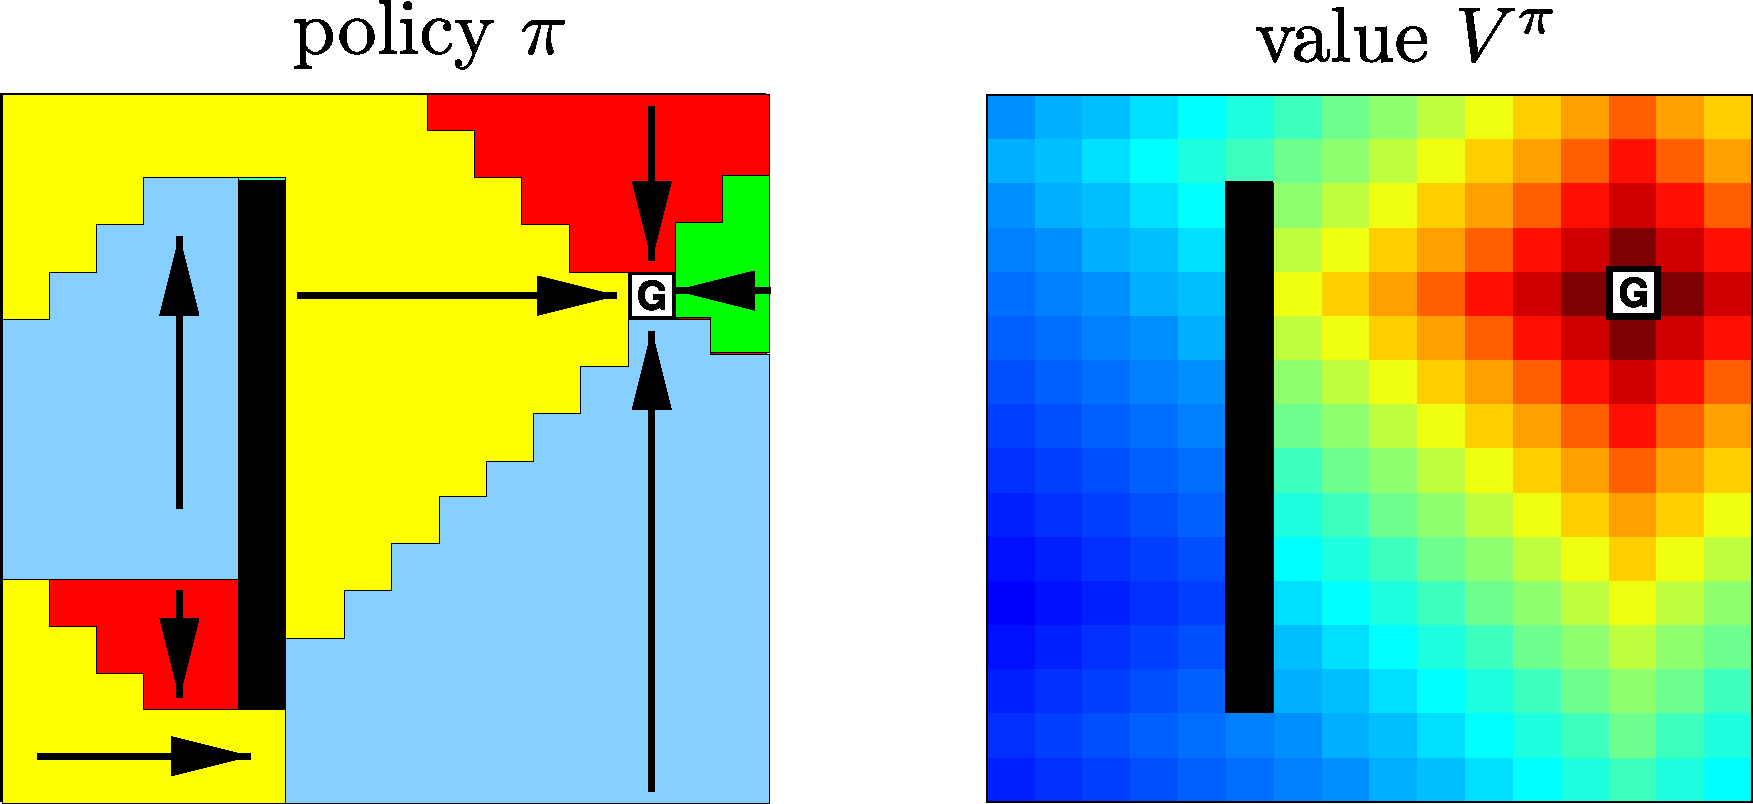
\includegraphics[trim={15cm 0 0 0mm},clip, height=3.5cm]{img/nav_policy_and_value} 
    \mode<article>{
    \captionof{figure}{
    Extract optimal policy from optimal value function
    }
    \label{fig:selectoptimalpolicy}
    } 
\end{center}

\pause

\slidesonly{\vspace{-5mm}}

\begin{equation}
\pi^{*}(\vec a_{k} | \vec x_{i}) = \argmax_{\vec a} \sum_{j=1}^{S} {\color{trans} P(\vec x_{j}| \vec x_{i}, \vec a)} \Big( {\color{reward}r(\vec x_{j}, \vec a)} + \gamma V^{*}(\vec x_{j}) \Big)    
\end{equation}   

\slidesonly{\vspace{-5mm}} 

\only<3>{
\question{What is going on here?}

\begin{enumerate}
%\item An optimal policy selects the action that maximizes this 
\item When at $\vec x_{i}$, look at the actions $\vec a$ that lead to all possible future states $\vec x_{j}$.
\item Select action $\vec a_{k}$ that maximizes the immediate reward + discounted successive value.
\end{enumerate}
}

\only<4>{
\question{What are the implications of selecting the optimal policy this way?}

\begin{itemize}
\item The above does not scale well for large state spaces.
\item The resulting $\pi^{*}$ is a \emph{greedy} policy, because it greedily selects using only the value function at hand. 
\end{itemize}
}

\end{frame}
